\documentclass[manuscript,review]{acmart}
\usepackage{graphicx} % Required for inserting images
\usepackage{url}
\usepackage{hyperref}
\usepackage{array, multicol, multirow}
\usepackage{booktabs}
\usepackage{subcaption} % side by side pic
\usepackage{amssymb}
\usepackage{algorithm}
\usepackage{algpseudocode}



\title{SAM 3D: 3Dfy Anything in Images}
\author{SAM 3D Team}\author{Xingyu Chen}\author{Fu-Jen Chu} \author{Pierre Gleize} \author{Kevin J Liang} \author{Alexander Sax} \author{Hao Tang} \author{Weiyao Wang}\author{Michelle Guo}\author {Thibaut Hardin} \author {Xiang Li} \author {Aohan Lin}\author{Jiawei Liu}\author{Ziqi Ma}\author{Anushka Sagar} \author{Bowen Song} \author{Xiaodong Wang} \author{Jianing Yang} \author{Bowen Zhang} \author{Piotr Dollár}\author{Georgia Gkioxari}\author {Matt Feiszli†} \author {Jitendra Malik}


\affiliation{\institution{Meta Superintelligence Labs}
\city{}
\country{USA}}

\date{July 2026}
\renewcommand{\shortauthors}{SAM 3D Team et al.}

\begin{document}

\begin{abstract}
    We present SAM 3D, a generative model for visually grounded 3D object reconstruction, predicting
geometry, texture, and layout from a single image. SAM 3D excels in natural images, where occlusion
and scene clutter are common and visual recognition cues from context play a larger role. We achieve
this with a human- and model-in-the-loop pipeline for annotating object shape, texture, and pose,
providing visually grounded 3D reconstruction data at unprecedented scale. We learn from this data
in a modern, multi-stage training framework that combines synthetic pretraining with real-world
alignment, breaking the 3D “data barrier”. We obtain significant gains over recent work, with at
least a 5 : 1 win rate in human preference tests on real-world objects and scenes. We will release our
code and model weights, an online demo, and a new challenging benchmark for in-the-wild 3D object
reconstruction.

\textbf{Code: }\url{https://github.com/facebookresearch/sam-3d-objects}

\textbf{Demo: }\url{https://www.aidemos.meta.com/segment-anything/editor/convert-image-to-3d}

\textbf{Website: }\url{https://ai.meta.com/sam3d}
\end{abstract}


\maketitle


\section{Introduction}
In our paper (see Figure \ref{overview}), we introduce an impressive new AI tool called SAM 3D, which can look at a single, everyday 2D photo and instantly build a fully complete 3D model of an object. Because our smart system recreates both the entire physical shape and the surface texture of the item, you can easily spin it around to view it from any desired angle, even if the original photo was highly cluttered or the object was partially hidden behind something else. Instead of needing pictures from multiple different angles like older computer programs typically do, SAM 3D works much more like the human brain. Psychologists and artists have actually known for a long time that humans can easily understand 3D depth just by looking at a flat image e.g. \citet{koenderink1992surfacep} in \citeyear{koenderink1992surfacep} demonstrated this elegantly by showing that humans can estimate surface normals at probe points on an object’s image, which can then be integrated to a full surface.

\begin{figure}[ht]
    \centering
    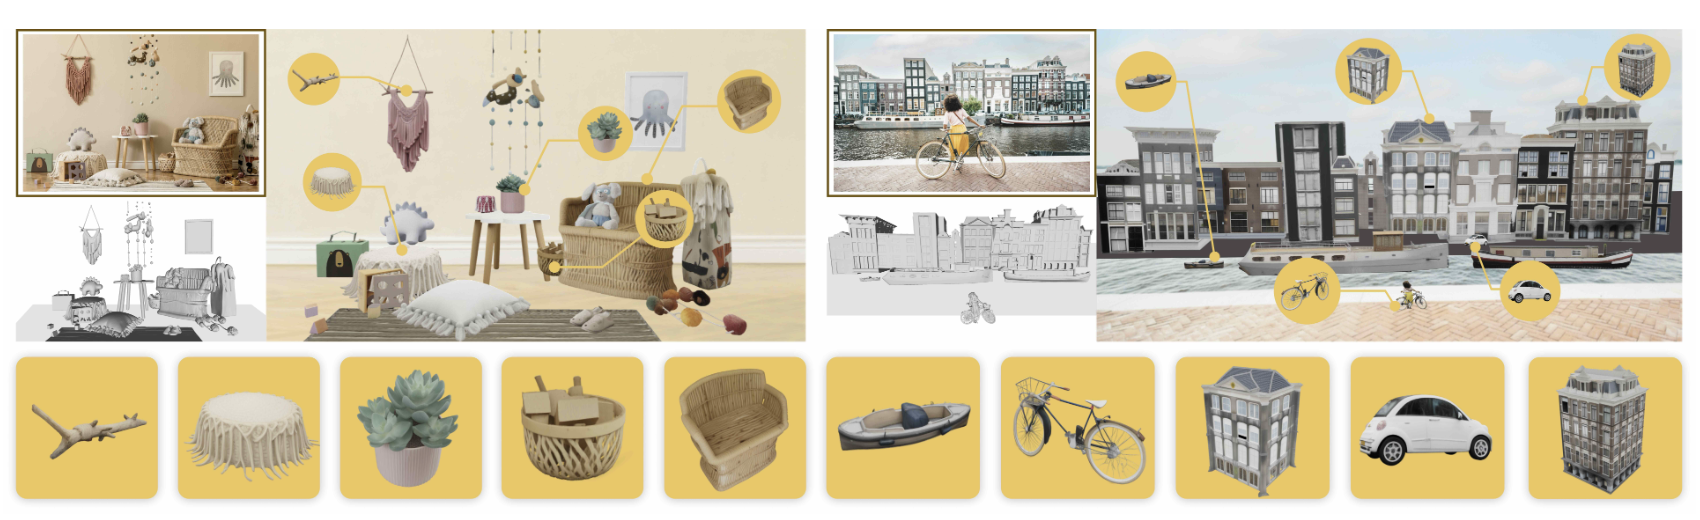
\includegraphics[width=0.9\linewidth]{1.png}
    \caption{\textbf{SAM 3D converts a single image into a composable 3D scene made of individual objects.} Our method predicts
per-object geometry, texture, and layout, enabling full scene reconstruction. Bottom: high-quality 3D assets recovered
for each object.}
    \label{overview}
\end{figure}

 Our AI mimics this natural ability by relying on simple visual clues—like how shadows fall, the patterns of textures, and recognizing familiar shapes—to understand how an object takes up space. By breaking things down into basic parts it has seen before, our AI can even accurately guess what the hidden sides of a brand-new, unseen object look like. However, the biggest hurdle we faced during development was a severe lack of good training data. To teach our AI to understand real life, we needed thousands of natural, everyday photos perfectly paired with exact 3D models. Older AIs were only trained on pictures of objects sitting completely alone on plain, blank backgrounds, which meant they would get totally confused and fail when trying to process messy, real-world scenes where objects are far away or heavily obscured by other things.wo insights made this possible:

 \begin{itemize}
    \item We can create synthetic scenes where 3D object models are rendered and pasted into images (inspired by \citet{dosovitskiy2015flownet} (\citeyear{dosovitskiy2015flownet})
    \item While humans can’t easily generate 3D shape models for objects, they can select the likely best 3D
    model from a set of proffered choices and align its pose to the image (or declare that none of the choices
    is good).
\end{itemize}

To train SAM 3D, we designed a step-by-step learning process inspired by how modern text AIs are trained \citet{minaee2025largelanguagemodelssurvey}, \citeyear{minaee2025largelanguagemodelssurvey}. We started with a pretraining phase using completely computer-generated objects to teach our model the basic vocabulary of 3D shapes and textures. Next, we moved to a mid-training phase where we pasted these 3D models into normal, everyday photos. Finally, we used a post-training phase to help the model adapt to entirely real images. Because everyday people cannot easily build 3D models from scratch to help us check the AI's work, we built a smart "model-in-the-loop" (MITL) system. Our system generates a few 3D shape guesses, and human helpers simply pick the best one and line it up, only sending the most difficult pictures to professional 3D artists. As these human helpers pick the best options, that correct data feeds back into our AI to make it smarter, which in turn helps it give better guesses the next time in a continuous cycle of improvement. Because there was not a good way to test this kind of real-world 3D AI before, we also created a brand-new testing set called SAM 3D Artist Objects (SA-3DAO). This dataset includes 1,000 pairs of real photos and perfect 3D models—ranging from massive churches and ski lifts to rare, everyday items—all hand-crafted by professional artists to set an expert human benchmark. We really hope that sharing this new evaluation tool will help speed up future research for everyone working on 3D reconstruction.


\begin{figure}[ht]
    \centering
    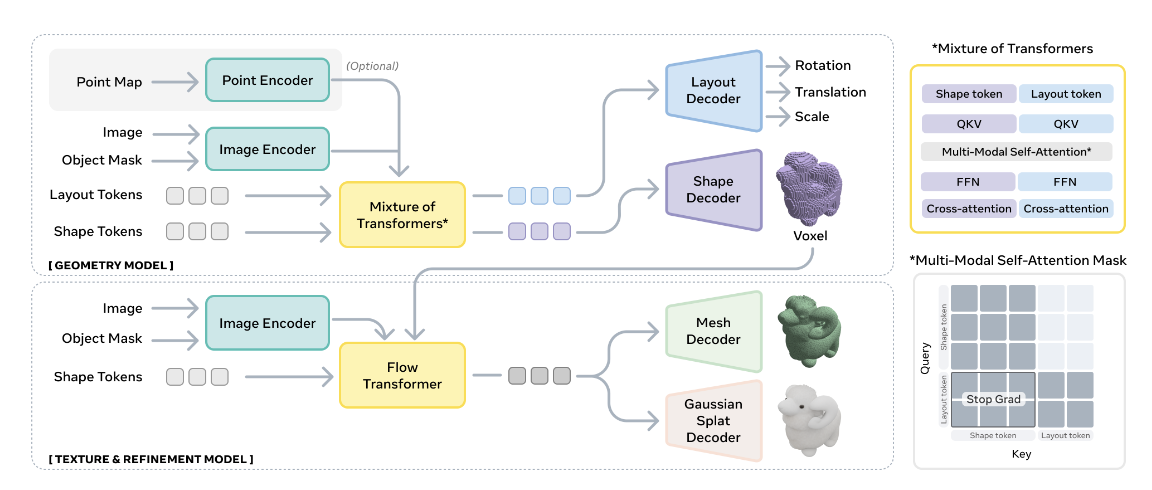
\includegraphics[width=1\linewidth]{2.png}
    \caption{\textbf{SAM 3D architecture.} \textbf{(top)} SAM 3D first predicts coarse shape and layout with the Geometry model; \textbf{(right)}
the mixture of transformers architecture apply a two-stream approach with information sharing in the multi-modal self-attention layer. \textbf{(bottom)} The voxels predicted by the Geometry model are passed to the Texture \& Refinement model, which adds higher resolution detail and textures.}
    \label{architecture}
\end{figure}

\newpage
We summarize our contributions as follows:
\begin{itemize}
    \item We introduce \textbf{SAM 3D}, a new foundation model for 3D that predicts object shape, texture, and pose from a single image. By releasing code, model weights, and a demo, we hope to stimulate further advancements in 3D reconstruction and downstream applications of 3D.
    
    \item We build a MITL pipeline for annotating shape, texture, and pose data, providing visually grounded 3D reconstruction data at unprecedented scale.

    \item We exploit this data via LLM-style pretraining and post-training in a novel framework for 3D reconstruction, combining synthetic pretraining with real-world alignment to overcome the orders of magnitude data gap between 3D and domains such as text, images, or video.

    \item We release a challenging benchmark for real-world 3D object reconstruction, SA-3DAO. Experiments show SAM 3D’s significant gains via metrics and large-scale human preference.
\end{itemize}

\section{The SAM 3D Model}
\subsection{Problem Formulation}

The act of taking a photograph maps a 3D object to a set of 2D pixels, specified by a mask $M$ in an image $I$. We seek to invert this map. Let the object have shape $S$, texture $T$ , and rotation, translation and scale$(R, t, s)$ in camera coordinates. Since the 3D to 2D map is lossy, we model the reconstruction problem as a conditional distribution $p(S, T, R, t, s|I, M ) $. Our goal is to train a generative model$ q(S, T, R, t, s|I, M ) $ that approximates p as closely as possible.

\subsection{Architecture}

We build upon recent SOTA two-stage latent flow matching architectures
\citet{xiang2025structured},\citeyear{xiang2025structured}. SAM 3D first jointly predicts object pose and coarse shape, then refines the shapes by integrating pictorial cues
(see Figure \ref{architecture}). Unlike \citet{xiang2025structured},\citeyear{xiang2025structured} that reconstructs isolated objects, SAM 3D predicts object layout, creating coherent multi-object scenes.

\textbf{Input encoding.} We use DINOv2 \citet{oquab2023dinov2}, \citeyear{oquab2023dinov2} as an encoder to extract features from two pairs of images, resulting in 4 sets of conditioning tokens:

\begin{itemize}
    \item \textbf{Cropped object:} We encode the cropped image I by mask M and its corresponding cropped binary mask, providing a focused, high-resolution view of the object.

    \item \textbf{Full image:} We encode the full image I and its full image binary mask, providing global scene context
and recognition cues absent from the cropped view. Optionally, the model supports conditioning on a coarse scene point map, P obtained via hardware sensors (e.g., LiDAR on an iPhone), or monocular depth estimation \citet{yang2024depth}, \citeyear{yang2024depth}\; \citet{wang2025moge}, \citeyear{wang2025moge}, enabling SAM 3D to integrate with other pipelines.
\end{itemize}

\textbf{Geometry Model.} This component predicts the conditional distribution $p(O, R, t, s \mid I, M)$. Specifically, it estimates the basic coarse shape ($O \in \mathbb{R}^{64^3}$) and the physical layout of an object---its 6D rotation ($R \in \mathbb{R}^6$) \citet{zhou2019continuity}\citeyear{zhou2019continuity}, translation ($t \in \mathbb{R}^3$), and scale ($s \in \mathbb{R}^3$) based on the input image ($I$) and mask ($M$) encodings. To achieve this, we use a 1.2-billion-parameter flow transformer built on a Mixture-of Transformers (MoT) architecture \citet{liang2025mixtureoftransformers}, \citet{deng2025Bagel}, which models the geometry and layout using the attention mask shown in Figure \ref{architecture}.

\textbf{Texture \& Refinement Model.} Once the rough shape is established, this model learns to add high-quality details and colors by modeling the distribution $p(S, T \mid I, M, O)$. We first extract the active voxels from the initial coarse shape and pass them through a 600-million-parameter sparse latent flow transformer. This step actively sharpens the geometry and synthesizes realistic object textures.

\textbf{3D Decoders.} Finally, the refined latent representations are translated into an actual 3D format. We use a pair of separately-trained VAE decoders ($D_m$ and $D_g$) that allow us to output the final object as either a standard 3D mesh or 3D Gaussian splats. Because they share the exact same VAE encoder, they operate perfectly within the same structured latent space \citet{xiang2025structured}\citeyear{xiang2025structured}.

\begin{figure}[ht]
    \centering
    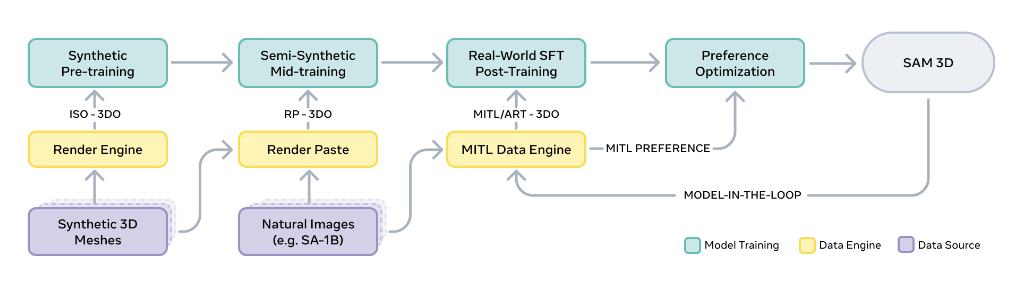
\includegraphics[width=1\linewidth]{3.png}
    \caption{\textbf{SAM 3D training paradigm}. We employ a multi-stage pipeline incrementally exposing the model to increasingly complex data and modalities.}
    \label{fig:3d training}
\end{figure}

\newpage

\begin{figure}[ht]
    \centering
    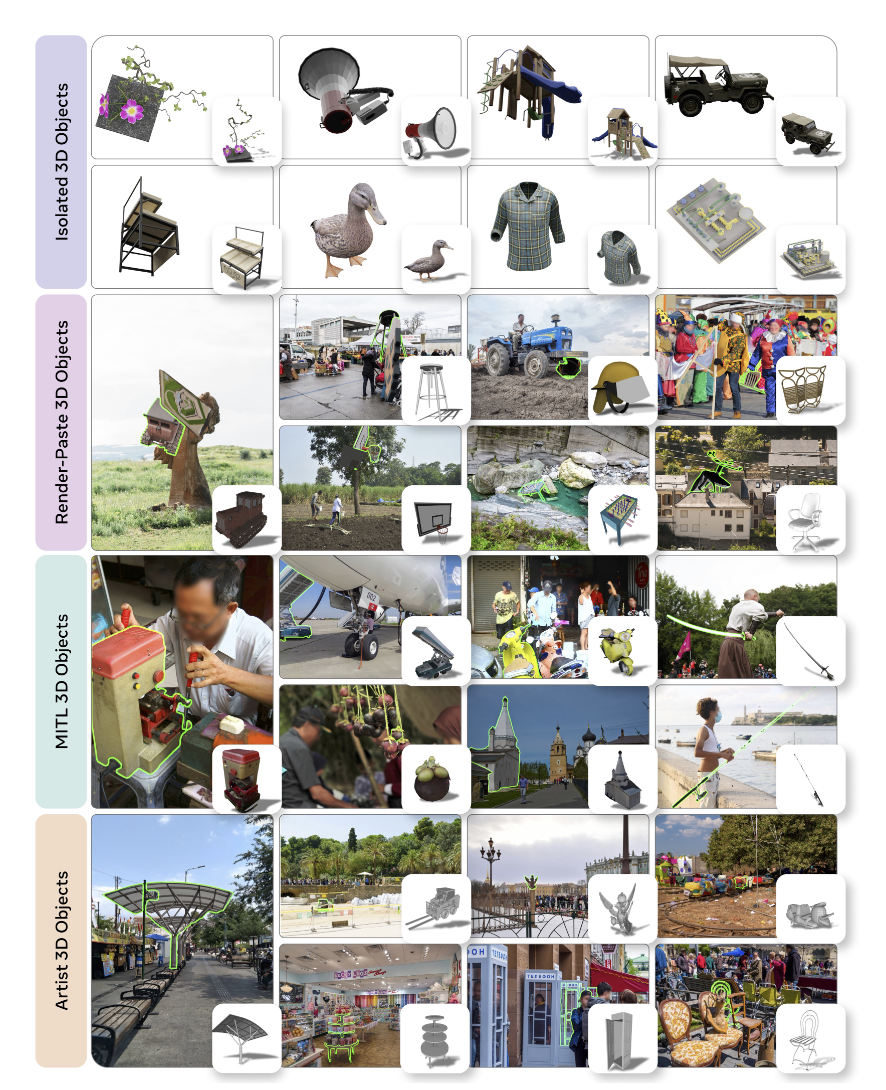
\includegraphics[width=1\linewidth]{big_pic.png}
    \caption{\textbf{SAM 3D data,}.with a green outline around the target object, and the ground truth mesh shown in the bottom
right. Samples are divided into four rows, based on type. Art-3DO meshes are untextured, while the rest may be textured or not}
    \label{fig:3d data}
\end{figure}




\clearpage

\section{Training SAM 3D}

SAM 3D breaks the 3D data barrier using a recipe that progresses from synthetic pretraining to natural post-training, adapting the playbook from LLMs, robotics, and other large generative models. We build capabilities by stacking different training strategies in pre- and mid-training, and then align the model to real data and human-preferred behaviors through a post-training data flywheel. SAM 3D uses the following approach:

\begin{itemize}
    \item \textbf{Step 1:} Pretraining. This phase builds foundational capabilities, such as shape generation, into a base model.Step 1.5: Mid-Training. Sometimes called continued pretraining, mid-training imparts general skills such as occlusion robustness, mask-following, and using visual cues.

    \item \textbf{Step 2:} Post-Training. Post-training elicits target behavior, such as adapting the model from synthetic to
real-world data or following human aesthetic preferences. We collect training samples $(I, M )$ $\rightarrow$ $(S, T, R, t, s)$ and preference data from humans and use them in both supervised finetuning $(SFT)$ and direct preference
optimization $(DPO)$

This alignment (step 2) can be repeated, first collecting data with the current model and then improving the
model with the new data. This creates a virtuous cycle with humans providing the supervision. Figure \ref{Impact of expanding training data} shows that as we run the data engine longer, model performance steadily improves; dataset generation emerges as a byproduct of this alignment. The following sections detail the training objectives and data sources used in SAM 3D. We focus on the Geometry model; Texture \& Refinement is trained similarly

\end{itemize}


\begin{table}[ht]
    \centering
    \begin{tabular}{l l l l}
    \hline
    \textbf{Training Stage} & \textbf{Modalities} & \textbf{Datasets} & \textbf{Conditional Input}  \\ \hline
    \multicolumn{4}{l}{\textbf{Stage 1 Geometry model}}\\ \hline
    \multirow{2}{*}{Pre-training} & $S, R$ & Iso-3DO & object-centric  crop\\
    & $S, R$ & RP-3DO & full image \\
    Mid-Training & $S, R, t, s$ & ProcThor, RP-3DO & full image, pointmap\\
    SFT & $S, R, t, s$ & MITL, Art-3DO  & full image, pointmap\\
    Alignment  & $S$ & MITL preference & full image, pointmap \\ \hline
    \multicolumn{4}{l}{\textbf{Stage 2 Testure \& Refinement model}}\\ \hline
    Pre-training & $T$ & Iso-3DO-500K & object-centric crop\\
    Mid-Training & $T$ & ProcThor, RP-3DO & full image, pointmap\\
    SFT & $T$ & MITL, Art-3DO  & full image, pointmap\\
    Alignment  & $T$ & MITL preference & full image, pointmap \\ \hline
    
    
    \end{tabular}
    \vspace{2\baselineskip}

    \caption{\textbf{SAM 3D training stages.} †Flying Occlusion (FO) from RP-3DO. ‡Object Swap - Random (OS-R) from RP-3DO. §Object
Swap - Annotated (OS-A) from RP-3DO.}
    \label{tab:training stages}
\end{table}

\subsection{Pre \& Mid-Training: Building a Base Model}

Teaching the AI starts in a simulated environment. By using massive datasets of computer-generated objects, the model learns the basics: shape, texture, and how objects sit in space. Building this strong foundation early means we do not have to spend as much time and money gathering expensive real-world data later. 

\subsubsection{\textbf{Pretraining: Single Isolated 3D Assets}}

First, we teach the AI using clean, isolated 3D models. We gathered 2.7 million 3D objects and rendered pictures of them from 24 different angles. This created a massive dataset, called Iso-3DO, of perfectly centered objects for the AI to study.

\subsubsection{\textbf{Mid-Training: Semi-Synthetic Capabilities}}

Next, we teach the AI how to handle messy, real-world scenes. We train it on three key skills:
\begin{itemize}
    \item \emph{Mask-following:} Focusing only on the specific object we highlight.
    \item \emph{Handling occlusions:} Guessing the shape of hidden parts when an object is blocked.
    \item \emph{Layout estimation:} Figuring out exactly where an object sits and how big it is.
\end{itemize}

To teach these skills, we created a "render-paste" dataset called RP-3DO. We did this by realistically pasting 3D objects into normal 2D photos, sometimes overlapping them (see Figure \ref{fig:3d data}). This lets the model practice on 61 million physically plausible scenes. However, because this data is still partially computer-generated, the AI requires a final round of training on purely real photos to truly bridge the gap to reality.

\begin{figure}[!h]
    \centering
    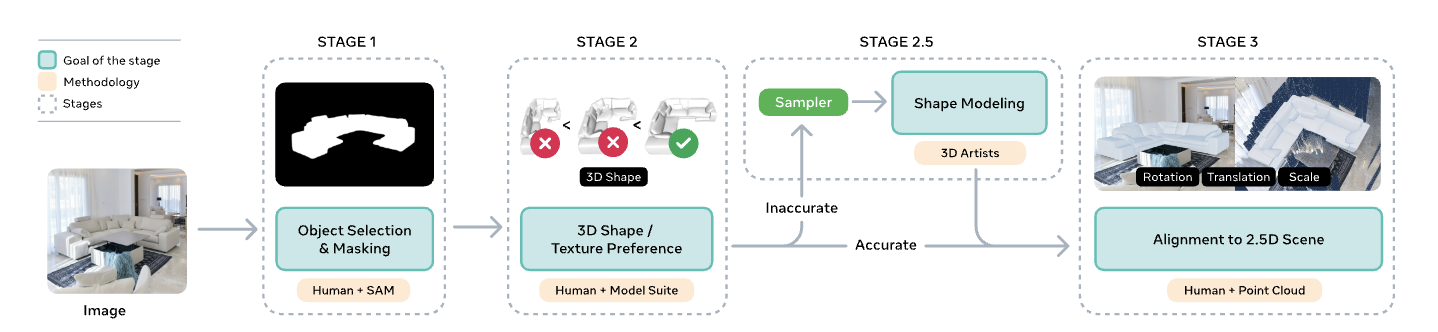
\includegraphics[width=1\linewidth]{4.png}
    \caption{\textbf{Life of an example going through the data collection pipeline.} We streamline annotation by breaking it into
subtasks: annotators first choose target objects (Stage 1); rank and select 3D model candidates (Stage 2); then pose these models within a 2.5D scene (Stage 3). Stages 2 and 3 use model-in-the-loop.}
    \label{fig:data collection pipeline}
\end{figure}

\subsection{Post-Training: Real-World Alignment}

Getting training data for 3D AI is incredibly difficult because normal people can't just build 3D models from scratch—it takes professional artists hours to make just one. However, the researchers realized something clever: while normal people can't make a 3D model, they are perfectly capable of picking the best one out of a lineup. This simple insight powers their entire data collection engine.

Here is the step-by-step pipeline they used to generate over 3 million 3D objects from almost 1 million real-world photos:

\textbf{Stage 1: Choosing target objects}$(I, M)$ The goal of this stage is to identify a large, diverse set of images $I$ and object masks $M$ to lift to 3D. They start by gathering a massive, diverse collection of real-world photos. Using a mix of human helpers and existing AI tools, they highlight specific objects (using masks) in those photos that they want to lift into 3D.

\textbf{Stage 2: Object model ranking and selectios}$(S, T)$ The goal of this stage is to collect image-grounded 3D shape $S$ and texture $T$ . The AI generates 8 different 3D shape and texture guesses for the highlighted object. Human annotators look at the lineup, pick the one that best matches the photo, and grade its quality.

If it's good, it becomes official training data. If it's bad, The bad guesses are kept and used to teach the AI what not to do in the future.

\textbf{Stage 2.5: Hard example triage (Artists).}: Calling in the Pros (Triage) Sometimes, an object is so complex or weird that all 8 AI guesses are completely unusable. Since regular human helpers can't fix these, these ultra-hard cases are sent directly to professional 3D artists to build perfectly from scratch.

\textbf{Stage 3: Aligning objects to 2.5D scene}:$(R,T,S)$ Setting the Scene (Layout) Just having a 3D shape isn't enough; the AI needs to know how it sits in the physical world. For the final step, human helpers take the winning 3D object and manually rotate, resize, and move it inside a virtual 3D space (using a point cloud guide) so its posture perfectly matches the original photo.

In general, we can think of the data collection as an API that takes a current best model, $q(S, T, R, t, s \mid I, M )$,and returns (i) training samples $D^+ = (I, M, S, T, R, t, s)$, (ii) a quality rating $r \in [0, 1]$, and (iii) a set of less preferred candidates $(D^- = (I, M, S', T', R', t', s'))$ that are all worse than the training sample.


\section{Experiments}


\textbf{Dataset.} To comprehensively evaluate the model capability under real-world scenarios, we carefully build a new benchmark \textbf{SA-3DAO1}\footnote{\url{https://ai.meta.com/datasets/sa-3dao-sam-3d-artist-objects}}, consisting of 1K 3D artist-created meshes created from natural images. We also include \textbf{ISO3D} from 3D Arena (Ebert, 2025) for quantitatively evaluating shape and texture, and Aria Digital Twin (ADT)(\citet{pan2023aria}, \citeyear{pan2023aria}) for layout. We further conduct human preference evaluation on two curated sets for both scene-level and object-level reconstruction. The \textbf{Pref Set} uses real-world images from MetaCLIP (\citet{xu2024amodal}, \citeyear{xu2024amodal}) and SA-1B (\citet{kirillov2023segment}, \citeyear{kirillov2023segment}), as well as a set based on LVIS (\citet{gupta2019lvis}, \citeyear{gupta2019lvis}). Refer to Section D for details on evaluation sets.

\vspace{1\baselineskip}

\textbf{Settings.} We conduct experiments with a Geometry model trained to condition on pointmaps. For datasets where pointmaps are unavailable, we estimate them with \citet{wang2025octothinkermidtrainingincentivizesreinforcement}, \citeyear{wang2025octothinkermidtrainingincentivizesreinforcement}. We found that shape and texture quality do not depend on whether the model is trained with pointmap conditioning (see Section E.5),but layout (translation/scale) evaluation in Table \ref{experiment table} requires ground-truth depth/pointmap as reference.


\begin{table}[!h]
    \centering
    \begin{tabular}{l c c c c c c }
\hline
      & \multicolumn{4}{c}{SA-3DAO} & \multicolumn{2}{c}{ISO3D Eval Set} \\ \hline
    Model & F1 @ 0.01 ($\uparrow$) & vIoU ($\uparrow$) & Chamfer ($\downarrow $)& EMD ($\downarrow$) & ULIP ($\uparrow$) & Uni3D ($\uparrow$)\\ \hline

    Trellis & 0.1475 & 0.1392 & 0.0902 & 0.2131 & 0.1473 & 0.3698 \\
    HY3D-2.1 & 0.1399 & 0.1266 & 0.1126 & 0.2432 & 0.1293 & 0.354\\ 
    6HY3D-2.0 & 0.1574 & 0.1504 & 0.0866 & 0.2049 & 0.1484 & 0.3662\\
    Direct3D-S2 & 0.1513 & 0.1465 & 0.0962 & 0.2160 & 0.1405 & 0.3653\\
    TripoSG & 0.1533 & 0.1445 & 0.0844 & 0.2057 & \textbf{0.1529} & 0.3687\\
    Hi3DGen & 0.1629 & 0.1531 & 0.0937 & 0.2134 & 0.1419 & 0.3594\\ \hline

    \textbf{SAM 3D} & \textbf{0.2344} & \textbf{0.2311} & \textbf{0.0400} & \textbf{0.1211} & 0.1488 & \textbf{0.3707}
\end{tabular}
\vspace{1\baselineskip}
    \caption{\textbf{3D shape quantitative comparison} to competing image-to-3D methods, including Trellis (Xiang et al., 2025), HY3D-2.1 (Hunyuan3D et al., 2025), HY3D-2.0 (Team, 2025), Direct3D-S2 (Wu et al., 2025a), TripoSG (Li et al.,2025), Hi3DGen (Ye et al., 2025). SA-3DAO shows metrics that measure accuracy against GT geometry; ISO3D (Ebert,2025) has no geometric GT and so we show perceptual similarities between 3D and input images (ULIP (Xue et al.,2023) and Uni3D (Zhou et al., 2023)). TripoSG uses a significantly higher mesh resolution, which is rewarded in perceptual metrics.}
    \label{experiment table}
\end{table}

\begin{figure}[ht]
    \centering
    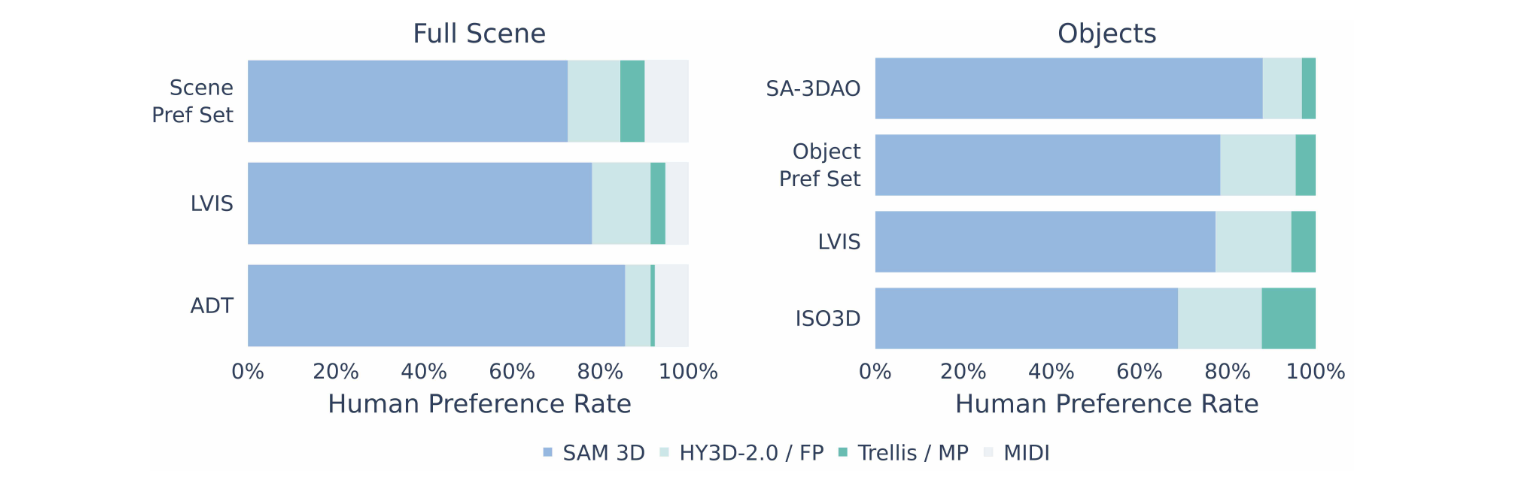
\includegraphics[width=1\linewidth]{5.png}
    \caption{\textbf{Preference comparison on scene-level and object-level reconstruction.} Numbers indicate human preference rates.
Objects comparisons are done on textured meshes. SAM 3D is significantly preferred over others on all fronts.}
    \label{fig:placeholder}
\end{figure}

\subsection{Analysis Studies}

\textbf{Consistent Gains from Post-Training}

As we continued to run our data engine, model performance steadily increased. This progress is reflected in the nearly linear rise in Elo scores during Stage 2 historical comparisons (Figure \ref{Historical Elo}). We discovered that it is crucial to scale all training phases simultaneously. This cumulative linear growth stems from a combination of running more data engine cycles, expanding both pretraining and mid-training, and introducing new post-training steps. While simply looping the MITL-3DO data by itself does yield steady gains, the benefits eventually start to taper off, showing a decreasing marginal impact (Figure \ref{Impact of expanding training data}).

\textbf{The Value of Multi-Stage Training}

SAM 3D's ability to handle real-world scenarios is a direct result of its phased training pipeline. As shown in Table \ref{multi-stage training}, the quality of 3D shapes improves almost continuously with the addition of each training phase, confirming the effectiveness of our approach leading to the final model (last row). We observe a similar positive trend for texture generation in the appendix . Additionally, Table 7 breaks down the specific impact of each real-world dataset by systematically removing the MITL-3DO, Art-3DO, or DPO stages to measure their individual contributions.



\section{Related Work}

\textbf{3D reconstruction} has been a longstanding challenge in computer vision. Classical methods leverage multiple views and include binocular stereopsis (\citet{wheatstone1838xviii}, \citeyear{wheatstone1838xviii}), structure-from-motion ( \citep{hartley2003multiple, szeliski2022computer, torresani2008nonrigid, tomasi1992shape}), and SLAM (\citet{smith1990estimating}, \citet{smith1990estimating}\; \citet{castellanos1999spmap}, 1999). Other strategies reconstruct by analysis (e.g., silhouettes (Esteban and Schmitt, 2004)) or by synthesis via volume rendering (\citet{kajiya1984ray}, \citeyear{kajiya1984ray}), using either implicit representations \citep{mo2025midtraininglargelanguagemodels} or explicit ones \citep{sitzmann2019deepvoxels, liu2020neural}. Supervised deep learning methods predict voxels \citep{xie2019pix2vox, wang2021multi} , point clouds \citet{van2022revealing}, \citeyear{van2022revealing}, or meshes \citet{worchel2022multi}, \citeyear{worchel2022multi}, or optimize implicit representations \citet{liu2022flow}, \citeyear{liu2022flow}, e.g., signed distance functions (SDFs), often with high-quality output but requiring multiple views at inference. In contrast, we focus on the more restrictive setting of a single RGB image at test time.

\vspace{2\baselineskip}

\begin{table}[ht]
    \centering
    \begin{tabular}{l c c c c c}
\hline
      & \multicolumn{4}{c}{SA-3DAO} & Preference Set \\ \hline
    Training Stage & F1 @ 0.01 ($\uparrow$) & vIoU ($\uparrow$) & Chamfer ($\downarrow $)& EMD ($\downarrow$) & Texture WR ($\uparrow$)\\

    Pre-training (Iso-3DO) & 0.1349 & 0.1202 & 0.1036 & 0.2396 & - \\
    $+$ Mid-training (RP-3DO) & 0.1705 & 0.1683 & 0.0760 & 0.1821 & 60.7\\
    $+$ SFT (MITL-3DO)& 0.2027 & 0.2025 &0.0578 &0.1510 &66.9\\
    $+$ DPO (MITL-3DO)& 0.2156 & 0.2156 &0.0498 &0.1367 &66.4\\
    $+$ SFT (Art-3DO) & 0.2331 & \textbf{0.2337} &0.0445 &0.1257 &-\\
    $+$ DPO (Art-3DO) & \textbf{0.2344} & 0.2311 &\textbf{0.0400} &\textbf{0.1211} &-\\
\end{tabular}
\vspace{1\baselineskip}
    \caption{\textbf{Cascading improvements from multi-stage training on 3D shape and texture.} For texture, we report win rates (WR) between each row and the row above it.}
    \label{multi-stage training}
\end{table}

\textbf{Layout estimation} extends single-instance estimation to full scenes. Instead of guessing a single massive 3D mesh for the whole room, our AI lets you use masks to select specific objects to reconstruct, and then it figures out both their shape and how they are positioned. Some past models tried to do this by guessing the shape first and then placing it in the scene, but we went with a "model-free" approach—like the one explored by \citet{brazil2023omni3d}, \citeyear{brazil2023omni3d} —where we estimate both the shape and the pose at the exact same time. While previous tools were typically stuck looking at simple tabletops or indoor floors, our approach works on a massive variety of object types across diverse environments.

\textbf{3D datasets.} Sourcing 3D annotations is challenging: it requires highly specialized skills. Anecdotally, it can take an experienced artist hours just to build one mesh from a single photo! Because of this, most existing large datasets (like Objaverse-XL; Deitke et al., 2023) are entirely computer-generated, meaning older models never really learned what real photos look like. The few real-world datasets that do exist are way too small or limited to basic indoor rooms (Reizenstein et al., 2021), leaving models trained on them struggling to generalize when faced with the real world.

\begin{figure}[ht]
    \centering
    % First Image
    \begin{subfigure}[b]{0.35\linewidth}
        \centering
        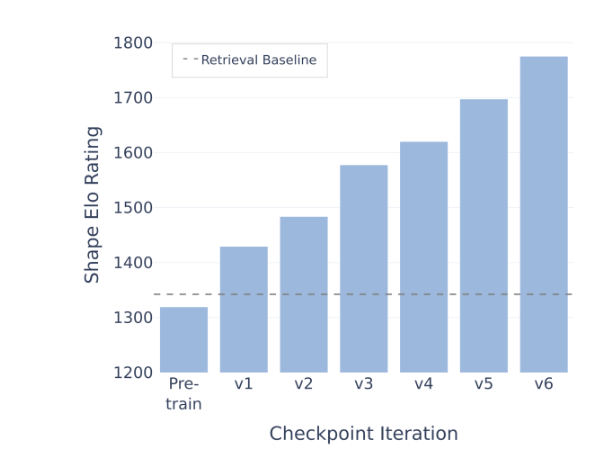
\includegraphics[width=\linewidth]{sub1.png}
        \caption{Historical Elo from data engine}
        \label{Historical Elo}
    \end{subfigure}
    \hspace{1 cm}
    % Second Image
    \begin{subfigure}[b]{0.35\linewidth}
        \centering
        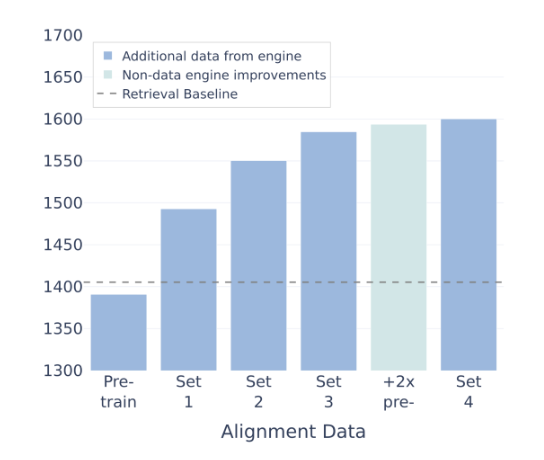
\includegraphics[width=\linewidth]{sub2.png}
        \caption{Impact of expanding training data}
        \label{Impact of expanding training data}
    \end{subfigure}

    \caption{Data engine with additional iterations. The plots show Elo scores of different models; a 400 point Elo difference corresponds to 10:1 odds in a preference test. Models were \textbf{\ref{Historical Elo}} checkpoints around 3 weeks apart, indicating cumulative
improvements as we scale and add different stages and \textbf{\ref{Impact of expanding training data}} post-trained (SFT) using expanded training data.}
    \label{fig: related works}        
\end{figure}

\textbf{Multi-stage pretraining.} Modern pretraining increasingly employs multiple training stages. Inspired by early ideas in curriculum learning (Bengio et al., 2009), we feed the model increasingly difficult and higher-quality data over time. Just like how other researchers use a dedicated "mid-training" phase to teach an AI a specific new skill like coding or expanding its memory \citet{rozière2024codellamaopenfoundation}, \citeyear{rozière2024codellamaopenfoundation}, we designed special pretraining and mid-training stages specifically tailored to teach our model how to master and generalize 3D shapes.

\section{Conclusion}
We share SAM 3D: a new foundation model for full reconstruction of 3D shape, texture, and layout of objects from natural images. SAM 3D’s robustness on in-the-wild images, made possible by an innovative data engine and modern training recipe, represents a step change for 3D and an advance towards real-world 3D perception.
With the release of our model, we expect SAM 3D to unlock new capabilities across diverse applications, such as robotics, AR/VR, gaming, film, and interactive media.


\bibliographystyle{plainnat}
\bibliography{biblio}

\end{document}
